%%%%%%%%%%%%%%%%%%%%%%%%
% $Autor: MansourAhmadyPhoulady, RanjeetsingTawar, HemanthPrabhakaran$
% $Pfad: Car_Licence_Plate_Identification_with_a_JetsonNano$
% $Version: 4.0.0 $
%
% !TeX encoding = utf8
%
%%%%%%%%%%%%%%%%%%%%%%%%



\chapter{Deployment}
\section{Deployment Pipeline}
\begin{figure}[h!]
	\centering
	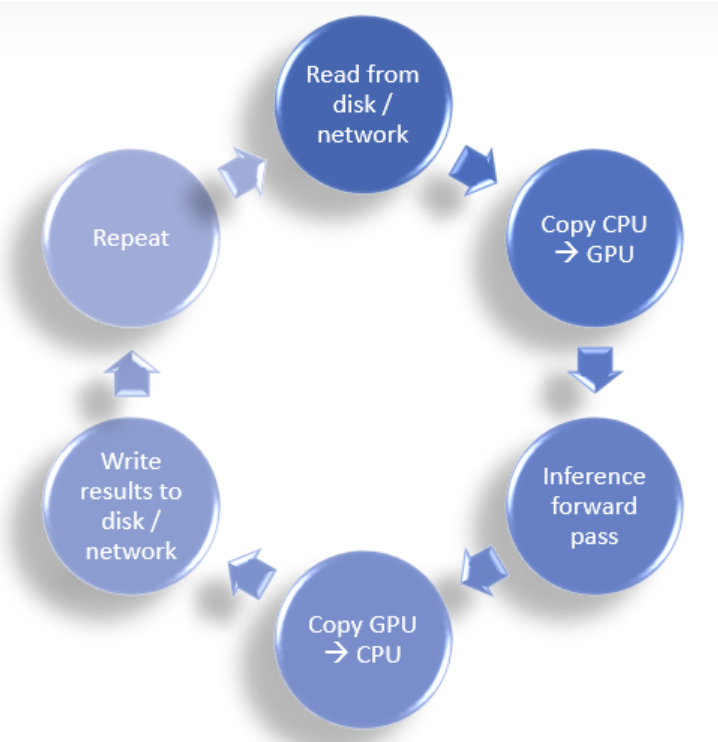
\includegraphics{Images/Deployment-process-flow}
	\caption{Deployment Process Flow}
\end{figure}
Deploy a trained custom model in jetson nano:

\subsection{Enhancing Model Execution on Jetson: A Runtime Optimization Guide}
It's important to note that JetPack versions are closely tied to TensorRT versions. This implies that the TensorRT checkpoints you have can only be utilized with the specific TensorRT version and JetPack version they were initially compiled on. For further details, you can refer to the NVIDIA developer’s forum for Jetson.

\subsection{Strategies for Identifying Optimal Production Parameters in Your Inference Workflow}
\subsubsection{Maximizing Model Efficiency: A Guide to Batch Size Selection on Jetson Devices}
Due to the limited memory space on Jetson, it's crucial to select a batch size that is modest enough to accommodate the constraints yet not so small that it adversely affects latency. For instance, in applications involving object detection, the optimal batch size should enable achieving a 30 frames per second (FPS) end-to-end performance. While working with GPUs typically involves aiming for a batch size between 1 and 64, the memory limitations and latency requirements of Jetson suggest keeping the batch size below 64.
Deci offers automated solutions to simplify this often lengthy and frustrating process. It is advisable to lean towards smaller batch sizes, particularly when dealing with large outputs. In some cases, using four replications of a batch size of 2 may outperform a single replication in a batch size of 8. Alternatively, leveraging the Deci Lab can provide insights into how your model performs with different batch sizes on Jetson devices.

\subsubsection{Optimizing Thread and Process Count for Efficient Model Execution}
Attaining the best configuration or a harmonious blend of these elements typically involves an iterative process of trial and error. It's essential for them to coexist seamlessly and collaborate to prevent any disruptions. Efforts should be directed toward automating this critical process to ensure optimal deployment on Jetson. Alternatively, leveraging Deci's optimization can help pinpoint the ideal balance for the number of threads and processes in your model.

\subsubsection{Evaluating Your End-to-End Pipeline: Beyond Inference Time Benchmarking}
The tasks are repetitive and consume time, adding to the overall inference duration. During benchmarking, it's crucial to assess applications comprehensively, encompassing not only inference time but also considering data transfer to and from the CPU, as well as pre- and post-processing stages.

\subsection{Jetson nano camera setup and python programming for OpenCV}
First, get USB camera formats from v4l2-ctl (provided by apt package v4l-utils). 

\begin{lstlisting}
	##Assuming the USB cam to be video node /dev/video1
	v4l2-ctl --device=/dev/video1 --list-formats-ext
\end{lstlisting}

Python code snippet to access the webcam:
\begin{lstlisting}
	import cv2
	cap = cv2.VideoCapture("/dev/video0", cv2.CAP_GSTREMER) 
	#check this
	print(cap.isOpened())
	while(True):
	#Capture frame-by-frame
	ret, frame = cap.read()
	#Our operations on the frame come here
	gray = cv2.cvtColor(frame, cv2.COLOR_BGR2GRAY)
	#Display the resulting frame
	cv2.imshow('frame', gray)
	if cv2.waitKey(1) & 0xFF == ord('q'):
	break
	# When everything is done, release the capture
	cap.release()
	cv2.destroyAllWindows()
\end{lstlisting}
\begin{figure}[h!]
	\centering
	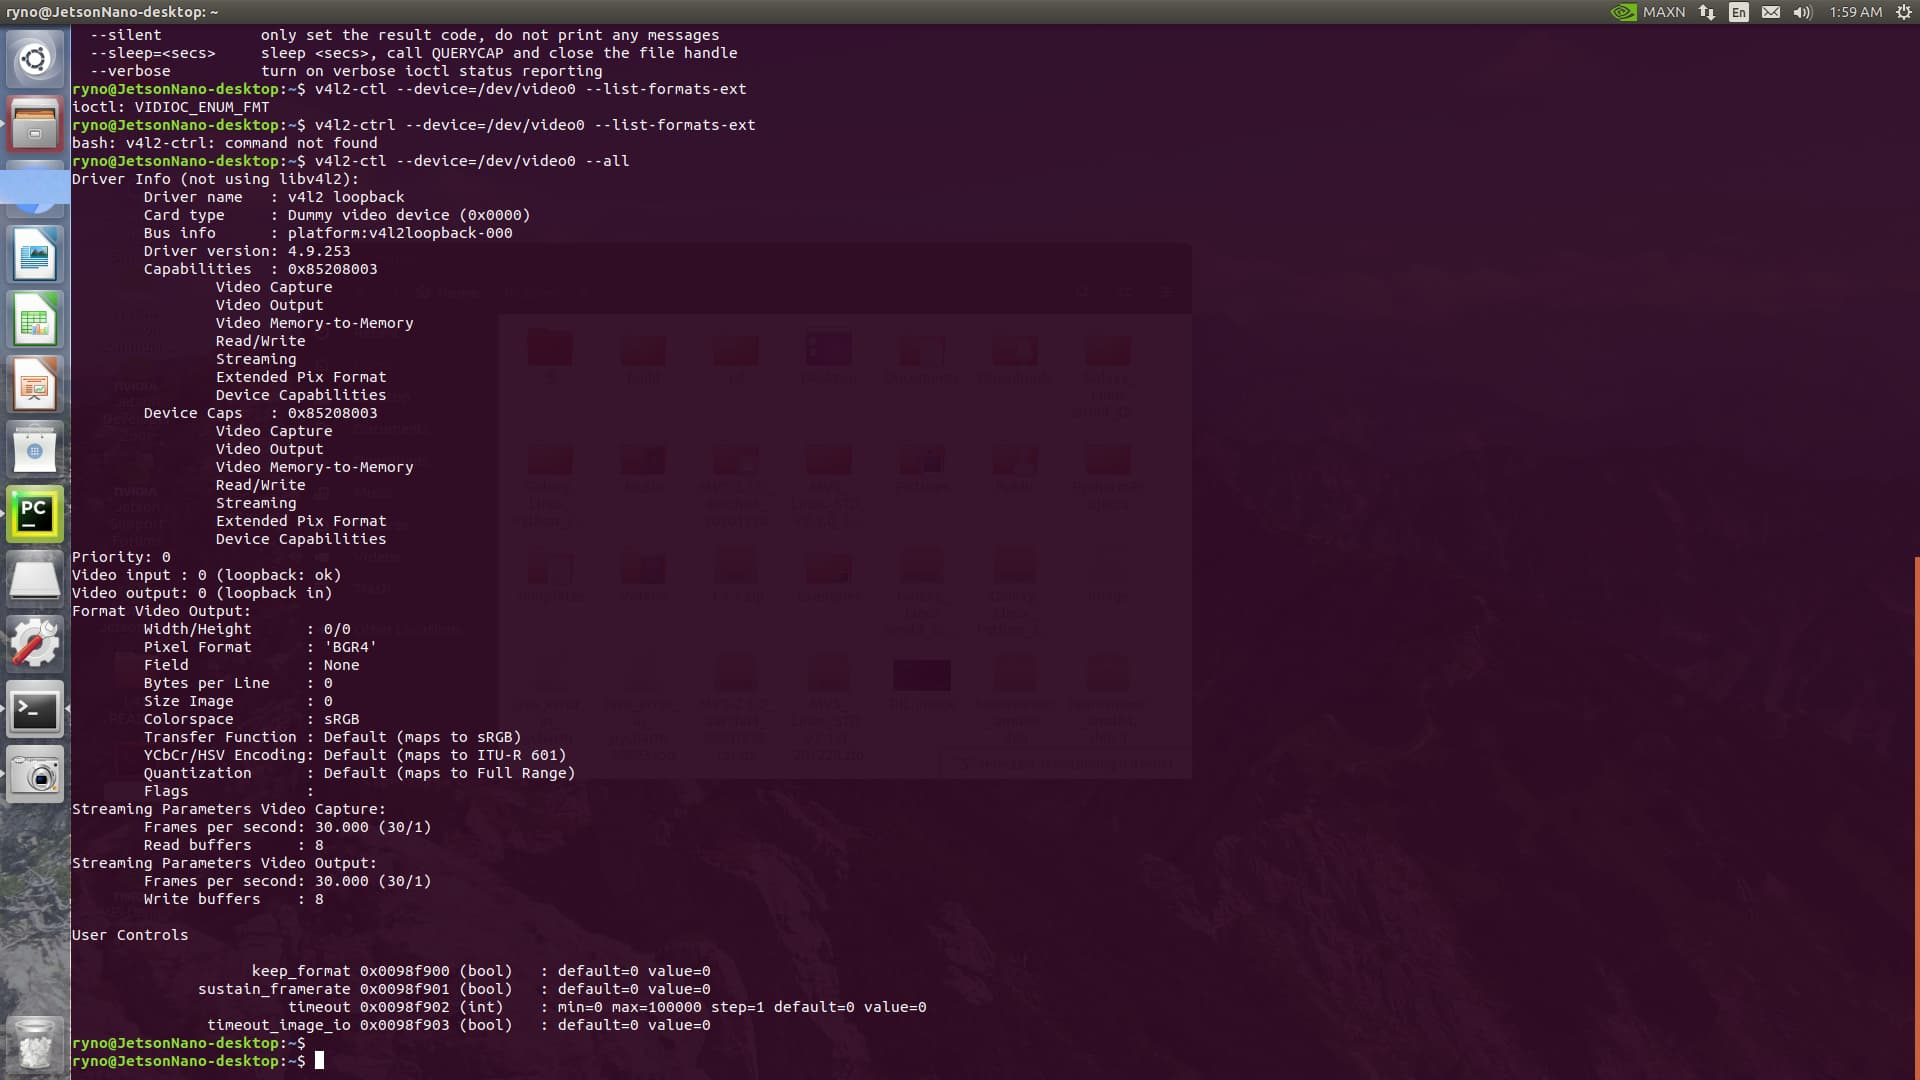
\includegraphics[width=\textwidth]{Images/jetson-nano-camera}
	\caption{Jetson Nano camera working}
\end{figure}
Opencv may read the camera from several capture backends, such as V4L or GStreamer. Before using Opencv, would try to get your camera feed into one of these backends. Check the SDK of a camera and see if it can provide a V4L interface or a GStreamer camera source plugin.

With OpenCV, the webcam operations are handled, for seamless object detection and object character recognition python code is written with jetson.inference, jetson.utils, import argparse, import sys libraries.

Application example: onnx PyTorch model for licence plate detection  detection with a combined data set of labels and images. The model trained in with combined labels and images shall be transformed into .onnx format and used on the Jetson Nano for image object detection.

This is intended to provide an example of a possible application of a network trained on the work PC on an edge computer in the field to enable the detection of a car licence plate in front of the camera. To do this, the previously trained model must be converted to .onnx and .engine files for use on the Jetson Nano.

Object detection module for car license plate detection:
Python code snippet for detection and Object Character Recognition:
\begin{lstlisting}
	import jetson.inference
	import jetson.utils
	import argparse
	import sys
	# parse the command line
	parser = argparse.ArgumentParser(description="Locate objects in a
	live camera stream using an object detection DNN.", 
	formatter_class=argparse.RawTextHelpFormatter,
	epilog=jetson.inference.detectNet.Usage()
	+jetson.utils.videoSource.Usage() + jetson.utils.videoOutput.Usage() 
	+ jetson.utils.logUsage())
	parser.add_argument("input_URI", type=str, 
	default="", nargs='?', help="URI of the input stream")
	parser.add_argument("output_URI", type=str, 
	default="", nargs='?', help="URI of the output stream")
	parser.add_argument("--network", type=str,
	default="ssd-mobilenet-v2", help="pre-trained model to load (see below for options)")
	parser.add_argument("--overlay", type=str, 
	default="box,labels,conf", help="detection overlay flags 
	(e.g. --overlay=box,labels,conf)
	\nvalid combinations are: 'box', 'labels', 'conf', 'none'")
	parser.add_argument("--threshold", type=float, 
	default=0.5, help="minimum detection threshold to use") 
	is_headless = ["--headless"] if sys.argv[0].find('console.py') != -1 else [""]
	try:
	opt = parser.parse_known_args()[0]
	except:
	print("")
	parser.print_help()
	sys.exit(0)
	# load the object detection network
	net = jetson.inference.detectNet(opt.network, sys.argv, opt.threshold)
	# create video sources & outputs
	input = jetson.utils.videoSource(opt.input_URI, argv=sys.argv)
	output = jetson.utils.videoOutput(opt.output_URI, argv=sys.argv+is_headless)
	# process frames until the user exits
	while True:
	# capture the next image
	img = input.Capture()
	# detect objects in the image (with overlay)
	detections = net.Detect(img, overlay=opt.overlay)
	# print the detections
	print("detected {:d} objects in image".format(len(detections)))
	#for detection in detections:
	print(detection)
\end{lstlisting}

\section{TensorFlow Lite}
%\chapter{Package \PYTHON{Example}}

\subsection{Introduction}

TensorFlow Lite is a „light“ version of TensorFlow designed for mobile and embedded devices. It achieves low-latency inference in a small binary size - both the TensorFlowLite models are much smaller. However, you cannot train a model directly with TensorFlow Lite, it must first be created with TensorFlow, and then you must convert the model from a TensorFlow file to a TensorFlow Lite file using the TensorFlow Lite converter. \cite{GoogleTensorFlow:2022}

\begin{figure}[h!]
	\centering
	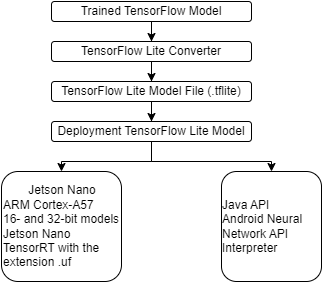
\includegraphics{Images/TFLite-ProcessFlow}
	\caption{TensorFlow Lite Process Flow \cite{GoogleTensorFlow:2022}}
\end{figure}

\subsubsection{Installation}
\begin{lstlisting}
	#TFLite
	#ONNX conversion is new, expect improvements as we support more ops.
	pip install tf2onnx
	python -m tf2onnx.convert --tflitessdmobilenet.tflite--output ssdmobilenet.onnx--opset13
	#Python Interface
	import tflite2onnx
	
	tflite_path = '/path/to/original/tflite/model'
	onnx_path = '/path/to/save/converted/onnx/model'
	tflite2onnx.convert(tflite_path, onnx_path)
	
	#Command line:
	tflite2onnx /path/to/original/tflite/model /path/to/save/converted/onnx/model
\end{lstlisting}

\subsection{Methodology}
Methodology utilized for TensorFlow Lite is as follows \cite{GoogleTensorFlow:2022}:
\begin{enumerate}
	\item \textbf{Develop Tensorflow CPU or GPU model in PC: }The model can be created from scratch and trained. The fine-tuned model is saved with the maximum accuracy and considered for deployment in TensorFlow Lite
	\item \textbf{Transformation of the model: }A custom model is used that is accordingly not in TensorFlow Lite format, it must be converted to the format using the 
	TensorFlow Lite Converter: Deployment on a target device: the TensorFlow Lite interpreter is available with APIs in many languages.
	\item \textbf{Further improvement of model: }TensorFlow Lite converter, Tensor-Flow models are converted into an optimised FlatBuffer format so that they can be used by the TensorFlow Lite interpreter
\end{enumerate}
\subsection{TensorFlow Lite Converter and Interpreter}
\subsubsection{Tensorflow Lite Converter}

tflite2onnx converts TensorFlow Lite (TFLite) models (*.tflite) to ONNX models (*.onnx), with data layout and quantization semantic properly handled.
Usage and ALPDR Model saved:
\begin{itemize}
	\item To convert a TensorFlow model (frozen graph *.pb, SavedModel or whatever) to ONNX, try tf2onnx. Or, firstly convert it to a TFLite (*.tflite) model, and then convert the TFLite model to ONNX.
	\item Microsoft has implemented another TensorFlow Lite to ONNX model converter in tf2onnx at Feb 2021. tf2onnx seems to able to convert Quantization, and it seems able to convert RNN networks which we are not supported yet. Please try tf2onnx --tflite if tflite2onnx missing any functionality.
	\begin{lstlisting}
		az\_ocr\_ssdmobilenetv1\_2.onnx.1.1.7103.GPU.FP16.engine
		az\_ocr\_ssdmobilenetv1.onnx
		az\_ocr\_ssdmobilenetv1\_3.onnx.1.1.7103.GPU.FP16.engine
		az\_ocr\_ssdmobilenetv1\_3.onnx
		az\_ocr\_ssdmobilenetv1\_2.onnx
	\end{lstlisting}
\end{itemize}


The TensorFlow Lite Converter is a tool available as a Python API that converts trained TensorFlow models into the TensorFlow Lite format. This is done by converting the Keras model into the form of a FlatBuffer, a special space-saving file format. In general, converting models reduces file size and introduces optimisations without compromising accuracy. The TensorFlow Lite converter continues to offer options to further reduce file size and increase execution speed, with some trade-offs in accuracy. \cite{GoogleTensorFlow:2022}
\subsubsection{Example Python Code}
\begin{lstlisting}
	saved_model_dir = '/content/TFLite'
	tf.saved_model.save(model, saved_model_dir)
	converter = tf.lite.TFLiteConverter.from_saved_model
	(saved_model_dir)
	tflite_model = converter.convert()with
	open('model.tflite', 'wb') as f:
	f.write(tflite_model)
\end{lstlisting}

\subsubsection{TensorFlow Lite Interpreter}

The TensorFlow Lite interpreter is a library that executes an appropriately converted TensorFlow Lite model using the most efficient operations for the given device, applying the operations defined in the model to the input and providing access to the output. \cite{GoogleTensorFlow:2022}

\subsubsection{TensorFlow Lite and Jetson Nano}
Often models are converted with Keras in the format HDF5 or with TensorFlow as a protocol buffer file with the extension .pb to a file in the format originally supported by TensorRT with the extension .uff to be used on the Jetson Nano. TensorFlow Lite is optimised for use on ARM CPU edge devices. Since the Jetson Nano also uses an ARM Cortex-A57 processor, using TensorFlow Lite on the Jetson Nano is an obvious choice.

\section{TensorFlow Lite for Microcontrollers}
\subsubsection{Introduction}
TensorFlow Lite has gained widespread adoption among mobile developers, but its engineering trade-offs didn't align with the requirements of all platforms. The team observed that many Google and external products could benefit from machine learning built on embedded platforms, where the existing TensorFlow Lite library fell short. The primary constraint was binary size, as even a few hundred kilobytes proved too large for these environments. They needed a solution that could fit within 20 KB or less. Additionally, many dependencies taken for granted by mobile developers, such as the C Standard Library, were absent. Consequently, code relying on these libraries couldn't be used. Despite these challenges, the requirements remained similar: inference as the primary use case, importance of quantized networks for performance, and a code base simple enough for developers to explore and modify were top priorities \cite{ten}.

\subsubsection{Work Flow}
\begin{enumerate}
	\item \textbf{Train a model:}
	\begin{itemize}
		\item Generate a small TensorFlow model that fits the target device and contains supported operations.
		\item Convert to a TensorFlow Lite model using the TensorFlow Lite converter.
		\item Convert to a C byte array using standard tools to store it in read-only program memory on the device.
	\end{itemize}
	\item \textbf{Run inference on the device using the C++ library and process the results.}
\end{enumerate}

\subsubsection{Installation}
\begin{lstlisting}[language=C++, caption={Installation code}, label={lst:installation_code}]
	#include "model.h"
	#include "tensorflow/lite/micro/kernels/micro_ops.h"
	#include "tensorflow/lite/micro/micro_error_reporter.h"
	#include "tensorflow/lite/micro/micro_interpreter.h"
	#include "tensorflow/lite/version.h"
	
	// Create an instance of the error reporter
	static tflite::MicroErrorReporter micro_error_reporter;
	
	// Define the tensor arena
	static constexpr int kTensorArenaSize = 2 * 1024;
	static uint8_t tensor_arena[kTensorArenaSize];
	
	// Create an instance of the interpreter
	static tflite::MicroInterpreter static_interpreter(
	model, tflite::MicroOpResolver::GetDefault(), tensor_arena,
	kTensorArenaSize, &micro_error_reporter);
	
	// Allocate memory for the input and output tensors
	TfLiteTensor* input = static_interpreter.input(0);
	TfLiteTensor* output = static_interpreter.output(0);
	
	// Perform inference
	static_interpreter.Invoke();
	
	// Print the output
	for (int i = 0; i < output->bytes; i++) {
		printf("%f ", output->data.f[i]);
	}
\end{lstlisting}

\subsubsection{TensorFlow Lite for Microcontrollers Example}

\begin{lstlisting}[caption={TensorFlow Lite for Microcontrollers Example}, label={lst:tf_lite_example}]
	import tensorflow as tf
	from tensorflow.lite.python import interpreter as tflite_interpreter
	
	# Load the TensorFlow Lite model
	model_path = "path/to/your/tflite_model.tflite"
	interpreter = tflite_interpreter.Interpreter(model_path=model_path)
	interpreter.allocate_tensors()
	
	# Get input and output details
	input_details = interpreter.get_input_details()
	output_details = interpreter.get_output_details()
	
	# Prepare input data (modify as needed)
	input_data = your_input_data
	
	# Set input tensor
	interpreter.set_tensor(input_details[0]['index'], input_data)
	
	# Run inference
	interpreter.invoke()
	
	# Get the output tensor
	output_data = interpreter.get_tensor(output_details[0]['index'])
	
	# Process the output (modify as needed)
	print("Inference result:", output_data)
\end{lstlisting}



